\documentclass[11pt]{article}
%\usepackage{imr}
%\usepackage{amssymb}
\usepackage{epsfig}

\def\thepage {}
%\bibliographystyle{imr}
%\newtheorem{Pseudo}{Pseudo-Code}[section]
\begin{document}

\title{\uppercase{Toward Interoperable Mesh, Geometry and Field Components for PDE Simulation Development}}
%\author{Lori Diachin$^1$ \and Mark Shephard$^2$}
%\thanks{
%$^1$ Center for Applied Scientific Computing, Lawrence Livermore National Laboratory, Livemore, CA 94551 \and
%$^2$ Scientific Computing Research Center, Rensellear Polytechnic Institute, Troy NY
%}
\date{Received: date / Revised version: date}

\maketitle
\begin{abstract}
abstract
\end{abstract}

\section{Introduction}

% \section{Introduction}

Requirements for modeling and simulation capabilities are increasing
in breadth of physics, fidelity of 
models, complexity of the systems to be simulated, problem size
(e.g. degrees of freedom) \cite{TACC}. These 
problems of interest are multi-physics and multi-scale in nature,
including electronic structures, seismic 
modeling, fusion, system biology, and climate modeling \cite{LLNL}.
The availability of supercomputers 
capable of sustained petaflops performance within the next several
years will create numerous opportunities 
to advance all these scientific applications by computer modeling of
previously intractable problems. The 
availability also challenges the current computer technologies and
algorithms, such as massively parallel 
computing and automatically adaptive simulations. 

In order to support scientific applications in SCOREC software framework at the petascale level, the system is 
required to satisfy the following items. 
\begin{itemize}

\item Balanced work loads on all processors. Even small imbalances
  result in many wasted processors. For 
example, 50,000 processors with one processor 5\% over average workload
				 is equivalent to 2380 idle
				processors 
and 47,620 perfectly balanced processors\cite{devine}.

\item Low interprocessor communication costs, including message
  passing volume and data redistribution costs. 
Processor speeds are increasing faster then network speeds.   

\item Scalable performance on computing algorithms, including scalable
  program execution time and memory 
usage on each processor. 
\end{itemize}

SCOREC has developed an entire software framework, including FMDB and ScorecMeshAdapt,  to 
support massively parallel adaptive, multiphysics and mutliscale
application codes, especially finite element 
method based applications. In the software framework, FMDB is
responsible for combining complex application-
independent capabilities into a single software infrastructure that is
shared by the application codes. 
ScorecMeshAdapt is responsible for parallel adaptivity for distributed,
unstructured meshes for the application codes. 

An overview of SCOREC software framework's capabilities and design abstractions of its
distributed dynamic object-oriented mesh 
data structure and parallel algorithms is presented in the following sections. These
capabilities include management of 
distributed mesh and field data structures, parallel mesh
input/output, interface to data 
partitioning and load balancing, and
transfer of data and fields between 
distributed meshes, and predictive load balancing for parallel
adaptive computations. 


%\begin{verbatim}
%1. Introduction
% - Motivation: there is a significant effort devoted to the development
%   of PDE solvers
%    - often this effort is somewhat peripheral to the main goals at
%      hand; that is the development of a new physics solver
%    - could be more effective if tools for the peripheral parts were
%      available for incorporation
%    - such tools would include automated meshing from general problem 
%      definitions, adaptive methods, multi-physics techniques
%
% - Even when they exist, simulation codes find it difficult to take 
%   advantage of these tools because of the current status of tool availability:
%    - libraries:
%        - typically focused; limited API options for accessing library
%          functionality
%        - difficult to experiment with different libraries that provide
%          similar capabilities (API is library specific)
%        - often don't interoperate with other libraries that provide 
%          related capabilities
%        - language interoperability often sketchy
%        - examples include F,G
%    - frameworks:
%        - typically impose structure on application code; reasonable
%          for new application development, but often difficult to rewrite
%          existing codes to conform
%        - simulation codes need to buy into the entire framework to use
%          the parts of most interest to them
%        - examples include X,Y
%
% - New work in scientific community focuses on the development of components 
%   which addresses some of the short comings of library or framework approaches
%    - Define a component (a software object meant to interact with other
%       components, encapsulating a certain functionality, clearly defined
%       interface and comforms to a prescribed behavior common to all components
%       in an architecture)
%    - Key: define a common API, multiple implementations/services that conform
%    - Useful in the following cases
%        - where there is a specialized analysis engine that cannot be easily 
%          reworked into a framework code and that requires multiple, related 
%          functionalities (perhaps provided by incompatible libraries)
%        - where experimentation with different techniques is of interest
%          (plug and play)
%        - where dynamic access to different, related services is required
%    - Other examples of work in this area
%        - CCA, solvers, etc
%    - TSTT work focuses on mesh/geometry/field tools - the focus of this paper
%\end{verbatim}

\section{Information Flow in Mesh-based simulation}
ITAPS uses the information flow through a mesh-based simulation to
guide the development of interoperable geometry, mesh and solution
field components.  While the information flow is modeled using the
requirements of a mesh-based PDE solver, the resulting components are
general enough to provide the infrastructure for a variety of other
tools including pre/post-processing of discrete data, mesh and
geometry manipulation, and error estimation.  A simulation's
information flow, depicted in Figure~\ref{fig:infoFlow}, begins with a
problem definition.  Described in more detail in
Section~\ref{sec:probDef}, the problem definition
%kkc 050613 includes the domain of the problem, 
%kkc 050613 the governing
%kkc 050613 mathematical form (PDEs, variational principle, etc) and any
%kkc 050613 parameters associated with the governing mathematics.  
consists of a description of the simulation's geometric and temporal
domain annotated by {\it attributes} designating mathematical model
details and parameters.
%kkc 050613 moved to 2.1 For example, a PDE solver may annotate the geometry with the
%kkc 050613 moved to 2.1 mathematical form governing the simulation (PDEs, variational
%kkc 050613 moved to 2.1 principle, etc) and any parameters associated with the governing
%kkc 050613 moved to 2.1 mathematics.  Other problem definitions (e.g. data analysis, adaptive
%kkc 050613 moved to 2.1 loops, mesh optimization, etc) may require additional or different
%kkc 050613 moved to 2.1 annotations.  
%Geometry representation %kkc 050613,  management 
%and attribute annotation form the central pieces of the problem definition.
%kkc 050613 Following problem definition
In the next stage of the information flow, mesh-based simulation
procedures approximate the PDEs by first decomposing the geometric
domain into a set of piecewise components, {\it the mesh}, and then
approximating the continuous PDEs on that mesh using, for example,
finite difference, finite volume, finite element, or partition of unity
methods.  Once the domain and PDEs are discretized, a number of
different methods can be used to solve the discrete equations and
visualize or otherwise interrogate the results.  Simulation automation
and reliability often imply feedback of the PDE discretization
information back to the domain discretization (i.e. in adaptive
methods) or even modification of the physical domain or attributes
(e.g., design optimization).  
%lad not sure this is useful info here
%Even when ITAPS components are not used to
%write the actual PDE solver, these components can be used to marshal
%information from the PDE solver back to the problem definition or
%domain discretization as part of a larger application such as an
%optimization or adaptive process.
%lad i don't think the following section adds anything at this point in
%    the text
%Information in the domain discretization, discussed in
%Section~\ref{sec:domainDisc}, is managed by mesh generation and mesh
%representation.  The geometry and mesh representations synergisticly
%form a conduit providing information to the other areas of the
%simulation: PDE discretization, solution and field interrogation.
%(Section~\ref{sec:pdeDisc}).   
The following sections present ITAPS' %kkc 050613 definition 
model of the information
flow in mesh-based simulations; these sections also introduce the
concepts of geometry, mesh and solution fields used to define ITAPS'
interoperable interfaces.

%\begin{figure}
%\begin{center}
%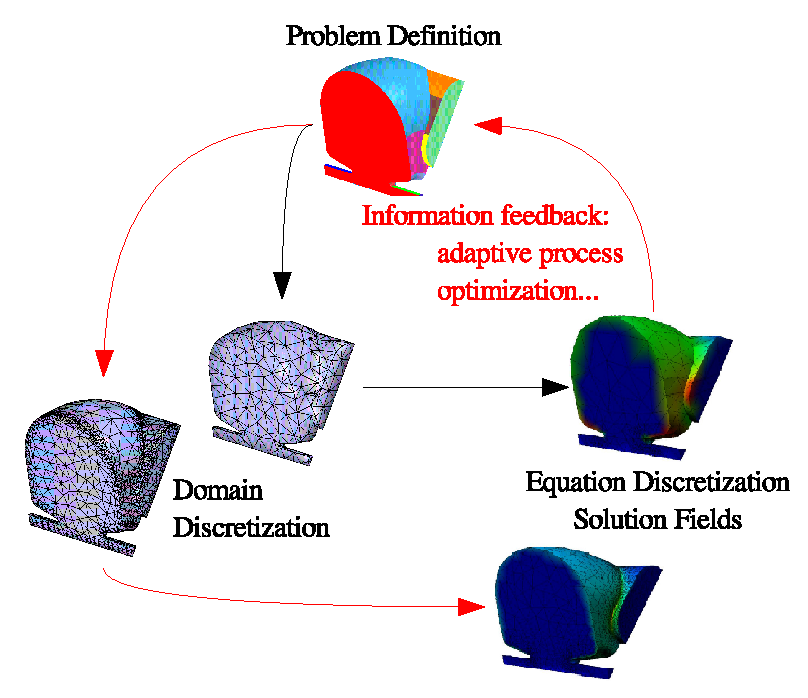
\epsfig{file=information_flow.eps,width=10cm}
%\caption{The information flow in a mesh-based simulation begins with
%a problem definition and continues through the domain and PDE
%discretizations.  Dynamic processes, such as solution adaptation and
%design optimization, require components capable of feeding information
%back to other parts of the information flow.}
%\label{fig:infoFlow}
%\end{center}
%\end{figure}

%kkc In mesh-based analysis procedures the PDEs are solved approximately
%kkc through a double discretization process in which the problem's
%kkc physical domain is discretized into a set of piecewise components
%kkc (e.g. a mesh) and the PDEs to be solved are discretized over the mesh
%kkc in an appropriate manner. The discretizations of the PDEs over the
%kkc mesh are assembled into a fully discrete system that is solved. The
%kkc result of this process yields the construction of a set of discretized
%kkc solution fields. Methods covered by such approaches include finite
%kkc difference, finite volume, finite element, boundary element and
%kkc partition of unity (so-called meshfree) methods.

\subsection{Problem Definition}\label{sec:probDef}

%kkc To qualify the operations and information involved in executing a
%kkc mesh-based simulation, we begin with a qualification of the problem
%kkc definition which includes:
%CFO-G We begin with a problem definition that qualifies the information (LAD
%CFO-G ???? WHAT DOES THIS MEAN?) and operators required by a mesh-based
%CFO-G simulation.  The problem definition includes:
%CFO-G 
%CFO-G Here's my swing at this one:
%kkc 050613 I like CFOG's sentence.
%% To identify the operations and information needed by a mesh-based
%% simulation, we begin with a problem definition containing:

%% \begin{itemize}
%% %I think this is more direct (cfog).  Also, moving it up puts the domain
%% %stuff together at the end for a nice transition to that topic...
%% \item The domain over which the simulation is to be performed. For the
%% classes of simulations being considered here the domain includes a
%% spatial component that is one-, two-, or three-dimensional and can
%% also include a temporal component if the solution changes with time.

%% %kkc 050613 \item The mathematical equations describing the physical processes to be
%% %kkc 050613 simulated (written as PDEs, variational principles, weak forms, etc).
%% %\item The mathematical form governing the simulation (e.g., PDEs,
%% %variational principles, weak forms).

%% \item Specification of %kkc 050613 parameters, referred to as 
%% physical {\it attributes} such as the %associated with including the governing
%% mathematical equations, material properties, forcing functions,
%% boundary conditions, and initial conditions.
%% \end{itemize}

%kkc 050613 rewrite the above description as single paragraph
To identify the operations and information needed by a mesh-based
simulation, we begin with a problem definition containing the {\it
domain} over which the simulation is to be performed and {\it
attributes} describing the problem that is to be solved.  For the
classes of simulations being considered here, the domain includes a
spatial component that is one-, two-, or three-dimensional and can
also include a temporal component if the solution changes with time.
To support a numerical simulation, the domain representation must be
able to support any geometry interrogation and/or modification
required by mesh generators and simulations, and the association of
mathematical and physical {\it attributes} with the geometry.  {\it
Attributes} specify the mathematical information required to solve a
particular problem.  This information includes, e.g., equations,
material properties, forcing functions, boundary conditions, and
initial conditions.  For example, a PDE solver may require a domain
definition annotated with the mathematical form governing the
simulation (PDEs, variational principle, etc) and any parameters
associated with the governing mathematical equations.  Other problem
definitions e.g., data analysis, adaptive loops, mesh optimization,
etc., may require additional or different attributes.

\begin{figure}
\begin{center}
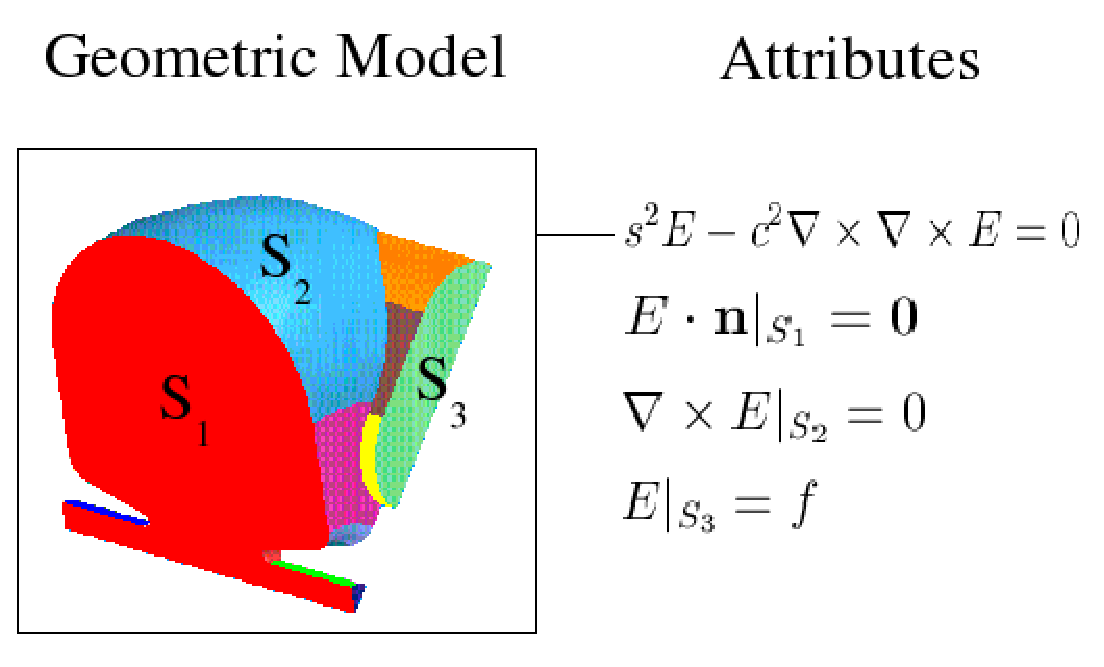
\epsfig{file=problem_description.eps,width=9cm}
\caption{The problem definition includes a geometric description of the domain
as well as attributes associated with geometric entities.  These attributes
are used to define the mathematical problem, its parameters and any other 
information needed by the simulation process.}
\label{fig:probDef}
\end{center}
\end{figure}

%\begin{itemize}
%\item Support the construction of a mesh that represents the domain
%discretization used in the simulation.

%\item Support any geometry interrogation required.
%\item any geometry interrogation and/or modification required by
%mesh generators and simulations, and

%\item the association of the physical and mathematical
%attributes with the geometry. %kkc ? mesh. cfog: concur

%\item Support the domain evolution in the cases where the domain
%changes as part of the solution process.
%\end{itemize}

\subsubsection{Geometric Domain}

%lad not sure this adds significantly to the bullets above
%lad Geometry interrogation and management supports the information flow at
%lad numerous points in a simulation.  Mesh generation and adaptation in
%lad particular rely upon geometric queries when discretizing the domain
%lad boundaries.  Physical models and discretizations require the
%lad information provided by attributes associated with the geometry.  For
%lad example, boundary conditions, initial conditions and constitutive
%lad models constitute information that can associated with the geometry.

%cfog What follows is a massive reordering of a couple of paragraphs to
%cfog avoid the issue, noted by Lori and/or Kyle, that we seem to be
%cfog dismissing CGM, image data, etc a bit too hastily.  Mostly I've
%cfog changed order, with some inevitable cleanup following.

%kkc 050613 I think we are still dismissing it, just less obviously now. (grep: more lines!)
%           The only way to support, for example, implicit or level set surfaces
%           with the current description would be to tesselate them 
%           and then compute a topological decomposition
%           of the triangulated surface (using methods referenced below).
%           The way I see it, non-b-rep geometry data is going to become more
%           important, not less.  The computer graphics folk seem to be heading
%           toward subdivision surfaces in a big way.  Again, those *could* be
%           used to construct a topological model; thus doing away with all the
%           nice features of subdivision methods.  Also, there have been many 
%           recent papers in siggraph (and such) on implicit surface modeling
%           Again, we only address this through firey hoops and assigning work 
%	    to others (hey, you come up with the algorithms).
%	    
%	    Why am I chewing on this bone?  Modeling biological and geophysical
%           processes (to name two up and comming cases) involve geometries
%           whose b-rep models are not available.  You can ask, but I am not sure
%           you will get an answer.  In EB applications we are seeing a lot
%           of implicit and level set surface definitions being used without needing
%	    the b-rep to generate the EB information.  These
%           representations are also useful for image data, MRI,CAT, and PET imaging.
%           Siesmograph modeling of subsurface features come in some form of
%           volume representation.  GIS data may come in triangulations
%           but I submit that any attempted topological decomposition of the Rockies would
%           be more confusing than a triangulation, not less.
%           
%           Is relying on the concept of a b-rep really a good long term strategy?
%           Not that I have an alternative yet, mind you, but maybe it is too
%           close to specifying an implementation... 
%	    YES, it is too late to bring this up. I only thought about it while editing the paper.
%	    
%	    
%	    At any rate, I think we need to have some answer; even if that answer
%	    is to convert the implicit/subdivision/voxel/etc data into a tesselated surface
%           which is then fed into a topology extraction algorithm.

%rev 1653:
%% Supporting geometry interrogation, modification and attribute
%% association requires a complete and flexible interface to the spatial
%% domain definition.  There are multiple approaches for defining the
%% spatial domain.  Computer aided design (CAD), image data and
%% cell-based (mesh-based) are among the most common geometry sources.
%% Each of these sources has one or more representational
%% forms. Historically, CAD systems use boundary representations. Image
%% data use a volumetric form such as voxels or octrees.  For cell-based
%% geometry, a variety of implicit and explicit boundary or volumetric
%% representations have been used.  Except in cases of image data and
%% when all aspects of the simulation process can be effectively defined
%% in terms of volumetric representations (e.g.  constructive solid
%% geometry, level sets, etc), it is generally accepted that the use of a
%% boundary representation is well suited for the spatial domain
%% definition.

%% WE JUST DISMISSED IMAGE, CSG, AND OTHER FORMS OF NON-BREP GEOMETRY.
%% DO WE REALLY WANT TO DO THAT...

%% A boundary representation (b-rep) consists of a collection of {\it
%% geometric entities}.  In this context, geometric entities are volumes,
%% surfaces, curves and points that collectively define a bounded portion
%% of three-dimensional space~\cite{mort97}; this bounded subset is
%% referred to as the {\it geometric model}.  There is substantial
%end rev 1653

Supporting geometry interrogation, modification and attribute
association requires a complete and flexible interface to the spatial
domain definition.  We consider {\it geometric models} that are subsets
of three-dimensional space bounded by a collection of {\it geometric
entities} (points, curves, surfaces, and volumes)~\cite{mort97}.  There
is substantial computer-aided design literature on various domain
representations.  Boundary representations (b-reps), which are the
most common geometric representation in CAD systems, are particularly
well-suited for geometric models as we define them.  Other domain
representations are also possible, including constructive solid
geometry; discrete (mesh-based) representations; and image data
(typically in the form of voxels or octrees).

For our purposes, details of how the geometric shape of the domain is
represented are immaterial.  We focus instead on the topological
abstractions to represent the geometric entities.  Topologically 3-, 2-,
1- and 0-dimensional entities are referred to as regions, faces, edges
and vertices, respectively.  Vertices form the boundaries of edges
(except in periodic edges, whose boundary set is null), edges bound
faces and faces are used to define regions.  The topological structure
of the geometric model is completely described by these entities and
their adjacencies.  The actual geometric information associated with a
geometric model entity, its shape, can be thought of as an attribute of
the entity.

The effective interaction of multiple domain definition sources
requires the definition of abstract interfaces that use information
that is common to all of them: that is, their topological entities.
%The ability to interact with
%topological entities provides an effective means to develop abstract
%interfaces allowing the easy integration to multiple domain definition
%sources.  
The ability to generalize these interfaces is further
enhanced by the fact that the geometry shape information needed by
most simulation procedures consists of pointwise interrogations that
can be easily answered in a method independent of the modeler shape
representation.  
%lad not sure what this adds
%lad The developers of CAD systems support geometry-based
%lad applications through general APIs.  These geometric modeling APIs have
%lad been successfully used to developed automate finite element modeling
%lad processes\cite{BeWa04,ShGe92}.

%lad too much detail
%lad An important consideration in the selection of a boundary
%lad representation is its ability to represent the classes of domain
%lad needed. In the case of numerical simulations the domains to be meshed
%lad can be general combinations of 0-, 1-, 2- and 3-D entities in general
%lad configurations. Figure~\ref{fig:non-man-model} shows a typical
%lad analysis domain that may be used for the structural analysis of a
%lad portion of a piping system. The analysis domain is an idealization
%lad where portions of the pipes are idealized by beams, the support
%lad bracket idealized by a plate and a full 3-D solid used for the pipe
%lad juncture.  The representation of such geometric domains, as
%lad well as others like multi-material domains, are referred to as a
%lad non-manifold boundary representations \cite{GuCh90,We88}. In the case
%lad of non-manifold models the representation must indicate how
%lad topological entities are used by bounding higher order entities. For
%lad example, each side of a face may be used by a different
%lad region. Therefore, faces have two uses. Another terminology for the
%lad use of a topological entity by higher order topological entities is
%lad co-entities \cite{Ta00}.

%% \begin{figure}
%% \begin{center}
%% \begin{pspicture}(-1,0)(11,6)
%% \rput(5,3){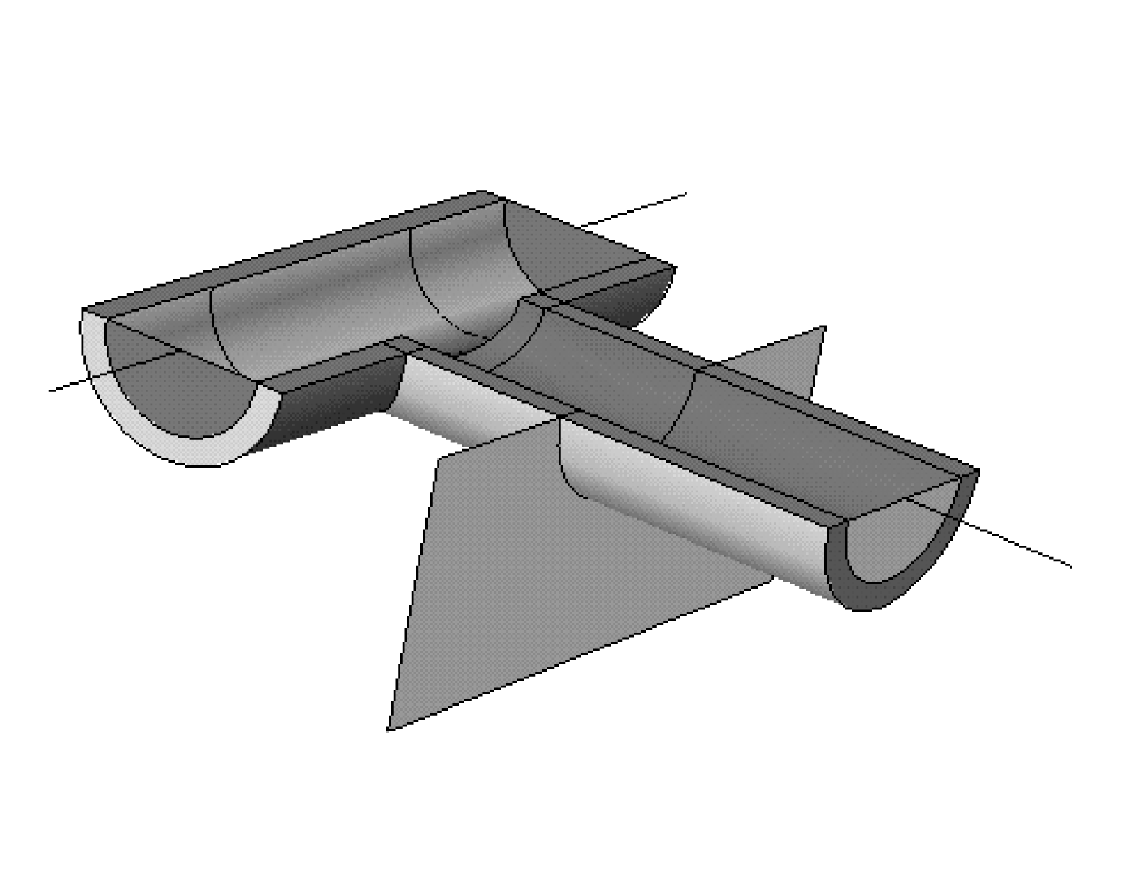
\epsfig{file=non-man-model.ps,width=9cm}}
%% \rput(4.2,.7){\makebox(0,0)[l]{\footnotesize support bracket (plate)}}
%% \rput(9.1,2.2){\makebox(0,0)[l]{\footnotesize pipe (beam)}}
%% \rput(6.,5.2){\makebox(0,0)[l]{\footnotesize pipe (beam)}}
%% \rput(1,3.2){\makebox(0,0)[r]{\footnotesize pipe (beam)}}
%% \rput(2.2,4.8){\makebox(0,0)[r]{\footnotesize junction (3-D solid)}}
%% %\psgrid
%% \end{pspicture}
%% \caption{A typical problem domain for the structural analysis of a piping system may use
%% geometric entities of different topological dimension for various
%% portions of the domain.  In this case, portions of the pipes are
%% idealized by beams, the support bracket idealized by a plate and a
%% full 3-D solid used for the pipe juncture.}
%% \end{center}
%% \end{figure}\label{fig:non-man-model}
%kkc Figure 1. Example of a non-manifold model used in simulation.

%ARE THE FOLLOWING TWO PARAGRAPHS REALLY RELEVANT TO THE INFORMATION FLOW????

%lad too much detail
%lad Geometric modeling systems maintain tolerance information on how
%lad numerically well the entities fit together.  This is necessitated by
%lad the fact that to function properly geometric modeling systems must
%lad employ finite tolerances.  The algorithms and methods within the
%lad geometric modeling system use the tolerance information to effectively
%lad define and maintain a consistent representation of the geometric
%lad model. (What many geometry-based applications have referred to as
%lad dirty geometry is caused by a lack of knowledge and proper use of the
%lad tolerance information \cite{BeWa04}.)

%lad Sometimes the only available domain representation is a mesh. Often it
%lad is still desirable to construct a high level topological
%lad representation of the problem domain. The process of constructing, or
%lad updating, the topological entities representing the domain geometric
%lad model is focuess on determining the appropriate subsets of the mesh to
%lad assocaiate with the model regions, faces, edges and vertices.
%kkc avoid ``mesh entities'' before introduction in the next section
%kkc is focused on determining the appropriate
%kkc sets of mesh regions, faces, edges, and vertices to associate with the
%kkc model regions, faces, edges and vertices respectively. 
%lad Algorithms to do this based on mesh based geometry and/or simulation
%lad contact or fracture information have been developed
%lad \cite{KrOr01,PaOr02,WaKo04}.  Once the model topology has been set,
%lad the geometric shape information can be defined in terms of the mesh,
%lad or can be made higher order \cite{CiOr00,OwWh01}.

%% kkc 050613 got rid of the next section since it has been supplanted by discussions
%%            in the problem definition introduction and geometric domain and attribute sections

%% \subsubsection{Governing Mathematics}

%% WE SHOULD DISCUSS SPECIFICIATION OF THE GOVERNING MATHEMATICS HERE.
%% WHAT IS THERE TO SAY?
%% HOW ABOUT :

%% LAD: I DON'T THINK THIS IS QUITE THE RIGHT INFORMATION AND I'M NOT HAPPY WITH
%% ATTRIBUTES BEING EVERYTING INCLUDING THE PDE.. IT SEEMS LIKE THERE SHOULD BE
%% SOME DISTINCTION - SO I WOULD LIKE TO TALK ABOUT BC, IC HERE - THEY ARE INTRINSIC
%% TO THE PDE - I WOULD WANT TO TALK ABOUT PARAMETERS BELOW - MATERIAL PROPERTIES
%% FOR EXAMPLE

%% The second aspect of problem definition are the governing mathematics.
%% A classical simulation tool's governing equations were built directly
%% into the structure and information flow of a code.  For example, a
%% time dependent PDE solver usually had a ``timestepping'' loop
%% surrounding the specific discretizations for the spatial part of the
%% PDE system.  Simulation frameworks often provide provide general
%% operators for discretizing PDEs that can be organized into codes
%% solving a particular problem~\cite{BrLa97,overtureTR,BeSh99}. Even
%% higher level approaches exist where interpreted languages or even
%% graphical interfaces are used to specify the high-level problem
%% definition.  Additional tools then translate this high level
%% specifiction into executable code by automatically assembling the
%% software components implied by the problem
%% definition~\cite{virtCell,pdeLab}.  ITAPS' component approach
%% addresses the first case, pre-exist information flow, by providing
%% common interfaces to information required by simulation codes.
%% Classical simulation tools can use ITAPS components to enhance or
%% expand their problem definitions without massive code development.
%% Simulation frameworks can use ITAPS tools to both expand the range of
%% problems they support as well as provide interfaces to their own
%% technology for use by other applications.  Finally, providing an
%% abstract interface to the information in the problem definition will
%% will allow high level interfaces access to alternative technologies
%% for domain representation and attribute association.  
%% UGH!!! STILL NOT HAPPY WITH THIS

\subsubsection{Attributes}
%kkc An examination of the properties of analysis attributes indicates they
%kkc are tensorial quantities \cite{BeSo83} that must be defined with
%kkc respect to a coordinate system. Generalized structures and methods can
%kkc define analysis attributes and associate them geometric model entities
%kkc\cite{OBSh02}.
Analysis {\it attributes} are information
associated with specific geometric entities in
the domain definiton.  In a PDE solver, these attributes include
the PDEs and initial conditions associated with a model region,
boundary conditions associated with boundary faces, and source terms
located within a model region.  Some attributes may be tensor-quantities %kkc 050613required by the problem definition and 
defined in various coordinate systems leading to the need for coordinate transformations
that allow other parts of the simulation process to access the data.
For example, a source term in the governing PDE is associated with a
geometric location in space and could be expressed using polar,
spherical or cartesian coordinates depending on the discretization.
%kkc 050613 not sure what else to say about attributes...

%One example could
%be a vector source term in the governing PDEs that is defined in
%spherical polar coordinates.  This source term would need to be
%transformed to Cartesian coordinates prior to use in a PDE
%discretization expressed in Cartesian coordinates.  
%kkc 050613 Generalized
%kkc 050613 structures and methods can define analysis attributes and associate
%kkc 050613 them with geometric model entities\cite{OBSh02}.  

\subsection{Domain Discretization}\label{sec:domainDisc}

The mesh is a piecewise decomposition of the space/time domain.  It is
common to employ different discretizations for the spatial and temporal
domains.  Because the definition of the spatial mesh is typically the
more complex of the two, it is the focus of this discussion.  In
addition to the case where a single mesh covers the entire geometric
(spatial) domain, we also consider cases where more than one mesh is
associated with a domain.  For example, in hybrid meshing approaches,
the domain is decomposed first into a set of sub-domains that may be
meshed using different meshing strategies.  Also, different full
geometry meshes can be used during different stages of the numerical
solution, as in the case of multilevel or adaptive methods.  In each of
these cases, the meshes can be associated with the underlying geometric
domain so that any changes made to the domain propagate properly to all
meshes.

\begin{figure}
\begin{center}
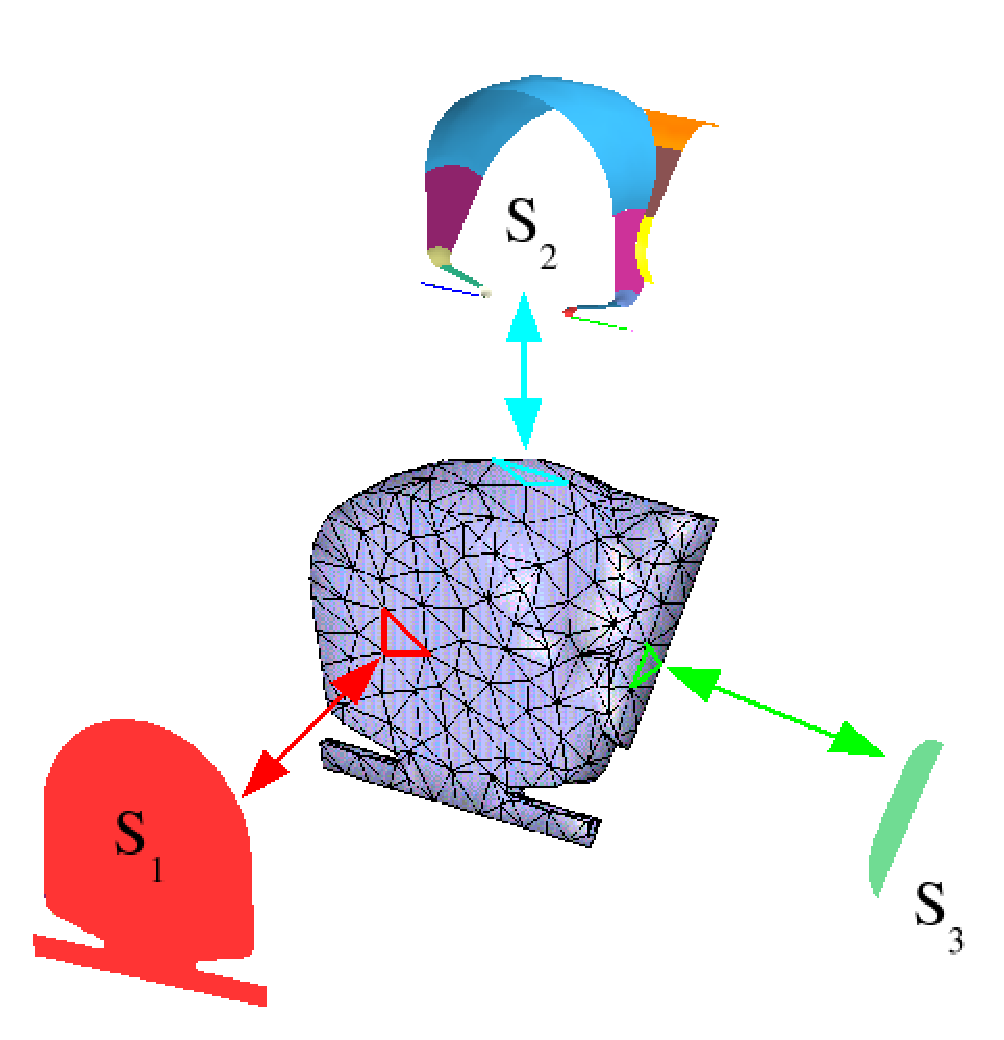
\epsfig{file=domain_discretization2.eps,width=8cm}
\caption{The domain discretization is a piecewise decomposition of the domain; usually a mesh.  Entities in the mesh (Vertices, Edge, Faces, and Regions) can
be associated with entities in the geometric model.  This association is referred to as ``classification'' of mesh entities on model entities.  Reverse classification associates model entities with mesh entities residing on that portion of the model.}
\label{fig:domainDisc}
\end{center}
\end{figure}

While different discretization approaches place different requirements
on the mesh and mesh entities, in general the mesh is required to
\begin{itemize}
\item have the appropriately defined union of the mesh
entities represent the domain of interest,
\item maintain, or have access to, the geometric shape information
needed for processes such as differentiation and integration,
\item support the PDE discretization process over the mesh entities, and
\item maintain relationships of the mesh entities needed to support
the assembly of the complete discrete system and construction of the
solution fields.
\end{itemize}

Meshes can take many different forms, the simplest of which is
a conforming mesh where the intersections of
two mesh entities is null and the intersections of their closure is
either null or the closure of a common boundary mesh entity (face,
edge or vertex). Other mesh forms include non-conforming meshes,
hierarchical, patch-based meshes, or overlapping meshes.
%lad where
%lad the intersections of the closure of two mesh entities is null, or
%lad different parts of the boundaries of the two mesh entities. Other mesh
%lad structures employ mesh patches that can interact in a variety of
%lad ways. Finally, other methods are defined in terms of overlapping
%lad regions (e.g. spheres or cubes). 
In each of these cases, there are
rules on how the mesh entities interact, how equation discretizations
are performed over them, and how the complete discrete system is
assembled.

%cfog Most of the following seemed to me to fit very well at the top of
%cfog the subsection.

%% THE FOLLOWING PARAGRAPH WAS MOVED FROM interface.tex TO HERE,
%% IT SHOULD BE WORKED INTO THIS SECTION

%% This domain must be decomposed into a set of mesh
%% entities. This process may employ a hierarchical decomposition of the
%% geometric domain. For example, the first level may decompose the
%% domain into a set of sub-domains that can be meshed using various
%% meshing strategies.  In particular, hybrid meshes consisting of
%% different component meshes can be used to discretize different
%% portions of the geometric domain, or different full geometry meshes
%% can be used during different stages of the numerical solution.  Each
%% of these meshes is associated with the full geometry domain so that
%% any changes made there propogate properly to the associated meshes.
%% Each mesh can be further decomposed into partitions for solution on a
%% massively parallel computer.

The geometric shape of the mesh entities is needed to support the
equation discretization process and can be effectively associated with
the topological entities defining the mesh. In many cases, this is
limited to the coordinates of the mesh vertices and, if they exist,
higher-order nodes associated with mesh edges, faces, or regions.  It
is also possible to associate other forms of geometric information
with the mesh entities, for example, associating Bezier curves and
surface control points with mesh edges and faces for use in {\it
p}-version finite elements \cite{LuSh02}.

It is possible to obtain mesh shape information by maintaining
an explicit link between mesh entities and a high-level description of
the geometric domain when it is available.  However, obtaining
information in this way is expensive and is often only used when
necessary.  Consider the case of mesh adaptation, the original domain
geometry must be used to ensure that the mesh approximates the
geometric domain to the same order of accuracy as the equation
discretization process approximates the continuous problem. For
example, as piecewise linear elements approximating curved portions of
the geometry are refined, the new mesh vertices must be placed on the
curved boundary, or as the polynomial order of an element is
increased, the geometric approximation of the closure of that entity
must be increased to the correct order.  If this high level geometric
information is not needed, for example, in the case of fixed mesh
simulations, it is typical to use only geometric shape information
associated directly with the mesh entities.

The data model for the mesh must maintain an association with the
domain definition, the discretization functions, the assembled
discrete system and the solution fields. From the perspective of
maintaining its relationship to the geometric domain, the use of
mesh topological entities and their adjacency is ideal
\cite{BeSh97,DeOB01,Ta00}. In this manner it is possible to associate
the mesh entities to the domain entities to obtain needed attributes
and geometric information.  In other cases, using topological entities
is not ideal.  For example, when using partition of unity (so
called meshfree) methods, an octree, or some other spatially-based
structure, is more appropriate. In the case of structured meshes
maintaining an explicit list of mesh entities is unnecessary; instead
one can maintain the boundaries of the mesh patches augmented with the
rules of mesh patch interaction.

We refer to the association of the mesh with respect to the geometric
model as {\it classification} \cite{BeSh97,ShGe92}. In particular, the
mesh topological entities are classified with respect to the geometric
model topological entities upon which they lie as defined below.

{\bf Definition: Classification} - {\it The unique association of mesh
topological entities of dimension $d_i$, $M^{d_i}_i$ to the
topological entity of the geometric model of dimension $d_j$,
$G^{d_j}_j$ where $d_i \leq d_j$, on which it lies is termed
classification and is denoted $M^{d_i}_i \sqsubseteq G^{d_j}_j$
where the classification symbol, $\sqsubseteq$,
indicates that the left hand entity, or set, is classified on the
right hand entity.}

{\bf Definition: Reverse Classification} - {\it For each model
entity, $G^d_j$ , the set of equal order mesh entities classified on that
model entity define the reverse classification information for that
model entity. Reverse classification is denoted as:}
\begin{equation}
RC(G^d_j) = \left\{ M^d_i | M^d_i \sqsubseteq G^d_j \right\}.
\end{equation}

The concept of mesh entity classification to a higher level model can
be extended to include additional levels of model decomposition. Two
important cases of this are parallel mesh partitions and structured
mesh partitions. In the cases when these partitions are
non-overlapping, the associations are obvious.  The concepts can be
extended to the case of overlapping partitions through the definition
of appropriate interaction rules for entities in the different models.

\subsection{Equation Discretization and the Definition of Solution Fields}\label{sec:pdeDisc}

The PDEs being solved are written in terms of dependent variables that
are functions of the space/time domain. Let the independent variables
of space be denoted ${\bf x}$, and the independent variable time be
denoted $t$.  For purposes of this discussion, let the set of
PDEs being solved be written in the form:

\begin{equation}
{\cal{D}}({\bf u}, \sigma) - f = 0
\end{equation}

where 
\begin{itemize}
\item $\cal{D}$ represents the appropriate differential operators,
\item $\bf{u} (\bf{x},t)$ represents one or more vector dependent variables,
\item $\sigma (\bf{x},t)$ represents one or more scalar dependent variables, and
\item $f (\bf{x},t)$ represents the forcing functions.
\end{itemize}
Note that the complete statement of a PDE problem must include a set
of boundary and, for time dependent problems, initial conditions.

In mesh-based PDE solvers, the dependent variables are discretely
represented over individual mesh entities or compact groups of entities,
either by direct operator discretization (e.g., difference equations) or
in terms of a set of basis functions. In both cases, this process
specifies a set of distribution functions defining how the discretized
variables vary over the mesh entities and a set of yet to be determined
multipliers, called degrees of freedom (DOF). The DOF can always be
associated with a single mesh entity while the distribution functions
are associated with one or more mesh entities.  Three common cases that
employ different combinations of interactions between the mesh entities,
the DOF, and the distributions are:
\begin{figure}
\begin{center}
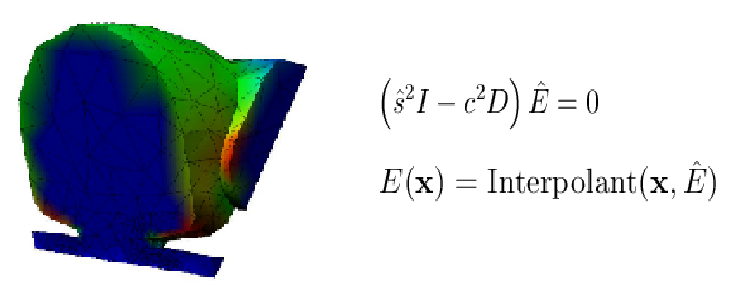
\epsfig{file=solution_fields.eps,width=8cm}
\caption{Solution fields provide access to simulation data and
discretizations.  In this example, $D$ is the discrete approximation
to the continuous system specified in the problem definition in
Figure~\ref{fig:probDef}.}
\label{fig:fields}
\end{center}
\end{figure}


%cfog:  I've inserted my own $0.02 here about the interpretation of
%cfog:  finite difference and finite volume methods.  Feel free to
%cfog:  change/debate my version as you see fit.

%kkc 050613 : thanks cfog, I concur with your changes.
\begin{description}
\item[{\it Finite difference methods.}]  In this case, the solution is 
represented by direct operator discretization: difference stencils are
written for all terms in the PDE.  These stencils are written in terms
of DOF that are the pointwise solution values for a compact collection
of mesh vertices.

\item[{\it Finite volume methods.}]  Finite volume methods compute the average
value of the solution in a set of control volumes that tesselate the
computational domain; these averages are the DOF.  Control volumes are
associated with mesh entities (vertices, edges, faces, or regions,
depending on the details of the scheme).  The distribution functions are
piecewise polynomials with discontinuities at control volume boundaries;
the coefficients of the polynomials are found using the DOF in
neighboring control volumes.


%cfog Mark:  I edited this paragraph a bit for length, considering that
%cfog it was longer than the finite difference and finite volume paras
%cfog combined.  I don't think I introduced any substantive errors in
%cfog the process, but it certainly bears checking.
\item [{\it Finite element methods.}]
Finite element distribution functions, referred to as shape functions,
are written over individual mesh entities, referred to as elements.  The
DOF represent values of the solution at particular points in the mesh
entity, refered to as nodes.  The shape functions associated with
neighboring elements can be made $C^m,~m \geq 0,$ continuous by having
common DOF associated with the shared lower-dimensional mesh entities.
In this case, the full set of DOF used by the element distribution
function can be associated with any of the mesh entities in the
closure of the mesh entity of the element.
\end{description}

Applying the discretization operation locally over the appropriate mesh
entities will produce a local contribution to the complete fully
discrete system.
%lad too much detail 
%lad The processes can be stated symbolically as:
%lad 
%lad \begin{equation}
%lad \cal{D} (\bf{D}^c, \bf{d}^c) - \bf{f}^c = 0 
%lad \end{equation}
%lad 
%lad where: 
%lad 
%lad \begin{itemize}
%lad \item $\cal{D}$ represents the discretized differential operators written in terms
%lad of appropriate distribution functions, $D^c$, over the domain of the
%lad contributor $C$ and $\bf{d}^c$ represents the vector of DOF associated with that
%lad contributor.
%lad 
%lad \item $\bf{f}^c$ represents the discretized representation of the known
%lad ``forcing functions'' and boundary conditions for that
%lad contributor.
%lad \end{itemize}
These can be combined to yield a discrete representation of the original
PDEs over the entire domain.
%lad that can be written as:
%lad 
%lad \begin{equation}
%lad \bf{k}^c \bf{d}^c = \bf{f}^c
%lad \label{eq:contrib_matrix}
%lad \end{equation}
%lad 
%lad where $\bf{k}^c$ is a matrix of parameters for contributor $C$ that multiple the
%lad vector of DOF associated with that contributor, $\bf{d}^c$.
%lad 
The construction of the system contributors can be controlled by the
appropriate traversal of information in the high-level problem
definition (e.g., the geometric domain), or at a level above the mesh
such as the mesh patch level for structured methods.

Note that the solution fields represent the variations of the tensor
variables over the domain of the problem. These fields
must be maintained in a form that is useful for queries
and manipulation as needed.  These manipulations include
the transfer of the fields to other meshes during a 
multiphysics analysis step, or to maintain the description
of the mesh on an adapted field.  Another common function that fields must
support is the construction of new fields through operations
that project the data onto new distributions with higher order
continuity, combine with other fields, etc..

%LAD NOT SURE THIS SECTION IS NECESSARY FOR INFORMATION FLOW
%lad \subsection{Discretized System Construction and Solution}
%lad 
%lad The relationship of the contributor level discretization given in
%lad (\ref{eq:contrib_matrix})
%lad to the complete discrete system is dictated by contributor level
%lad mappings that ``map'' the contributor level DOF to the
%lad ``assembled'' vector of the DOF for the complete system, $\bf{d}$. The
%lad process of constructing the complete system from the contributors is
%lad referred to as the assembly process. Symbolically the complete
%lad discrete system can be written as:
%lad 
%lad \begin{equation}
%lad \bf{K} \bf{d} = \bf{F}
%lad \end{equation}
%lad 
%lad where
%lad 
%lad \begin{itemize}
%lad \item $\bf{K}$ is a system level matrix of parameters.
%lad \item $\bf{d}$ is the complete vector of DOF 
%lad \item $\bf{F}$ is the complete right hand side vector.
%lad \end{itemize}
%lad 
%lad Symbolically the relationship between the contributor level and system
%lad level matrices and vectors can be depicted as:
%lad 
%lad \begin{equation}
%lad \bf{d} ~=~ A^{N_c}_{c=1}(\bf{d}^c),~K~=~A^{N_c}_{c=1}(\bf{k}^c),~\bf{F}~=~A^{N_c}_{c=1}(\bf{f}^c)
%lad \end{equation}
%lad 
%lad where 
%lad \begin{itemize}
%lad \item $N_c$ is the number of contributors in the complete system
%lad \item $A^{N_c}_{c=1}$ indicates an assembly operator that is applied to each
%lad contributors contributions and properly maps it to the complete
%lad discrete system.
%lad \end{itemize}
%lad 
%lad There are a variety of specific representational forms for the
%lad complete systems matrices.  The specific form used is function of the
%lad methods used to perform the computationally intensive process of
%lad solving the discrete system to determine the values of the system DOF.
%lad The global algebraic equations are solved to produce the values of the
%lad system DOFs. Once the system level DOF are determined, the mappings
%lad between the contributor level and system level DOF can be used to
%lad complete the specification of the solution fields.


% LocalWords:  ITAPS interoperable PDEs KKC meshfree PDE TSTT's


%\begin{verbatim}
%  - Gives the overview of PDE simulation steps - based on the general 
%    discretization docuement from last summer (Mark, can you send that out again?)
%  - Assumptions and definitions
%      - Mesh:  high level view of data model, functionality expected
%      - Geom:  high level view of data model, functionality expected
%      - Field: high level view of data model, functionality expected
%      - Others?
%  - How they are related to each other
%\end{verbatim}

\section{The TSTT Interface Definition efforts}

To support the flow of information in mesh-based simulations a number
of tools and technologies have been developed by different research
groups in academia, industry and the government labs.  For these tools
to have maximum impact it is important that they be interoperable,
interchangeable, and easily inserted into existing application
simulation codes.  Accomplishing this goal will allow easier
experimentation with different, but functionally similar, technologies
to determine which is best suited for a given application.  In
addition, it will provide mechanisms for combining technologies
together to create hybrid solution techniques that use multiple
advanced tools.

To accomplish this goal, we have defined an abstract data model that
encompasses a broad spectrum of mesh types and usage scenarios {\it
and} a set of common interfaces that are implementation and data
structure neutral.  The set of interfaces must be both small enough to
encourage adoption but also flexible enough to support a broad range
of mesh types.  {\it LAF should we move this figure and discussion to
section 2?} Figure \ref{fig:hieracrhy} shows the hierarchical
relationship between the geometric description of the computational
domain and first discretization step in PDE-based simulation.  At the
highest level is the geometric description of the computational domain
which can be decomposed into different parts that can be meshed using
various meshing strategies.  In particular, hybrid meshes consisting
of different component meshes can be used to discretize different
portions of the geometric domain, or different full geometry meshes
can be used during different stages of the numerical solution.  Each
of these meshes is associated with the full geometry domain so that
any changes made there propogate properly to the associated meshes.
Each mesh can be further decomposed into partitions for solution on a
massively parallel computer.

The TSTT data model abstracts this simulation data hierachy and is
decomposed into three {\it core data types}: the geometric data, the
mesh data, and the field data.  These core data types are associated
with each other through {\it data relation managers}. The data
relation managers control the relationships among two or more of the
core data types, resolve cross references between entities in
different groups, and can provide additional functionality that
depends on multiple core data types.  Work on the mesh data model and
API has progressed the farthest and we describe it some detail in
Section \ref{sec:mesh}.  Preliminary work on the geometry and field
data model and interfaces are discussed as well.

A key aspect of this approach is that we do not enforce any particular
data structure or implementation with our interfaces, only that
certain questions about the mesh, geometry or field data can be
answered through calls to the interface.  To encourage adoption of the
interface we aim to create a small set of interfaces that existing
mesh and geometry packages can support.  The latter point is critical.
The DOE, NSF, DoD and other federal agencies have invested hundreds of
man years in the development of a wide variety of geometry, mesh
generation and mesh management toolkits.  These software packages will
not be rewritten from scratch to conform to a common API, rather the
API must be data structure neutral and allow for a broad range of
underlying mesh representations. However, only a small set of
functionalities can be covered by a 'core' set of interface functions.
To increase the functionality of the TSTT interface, we define
additional, optional, interfaces for which we will provide reference
implementations based on the core interface methods.  Developers can
be implement these functions on their own mesh database as needed.
The allows for incremental adoption of the interface.

One of the foremost challenges inherent in this type of effort include
balancing performance of the interface with the flexibility needed to
support a wide variety of mesh types.  Performance is critical for
kernel computations involving mesh access.  To address this need we
provide a number of different access patterns including array and
iterator-based.  The user may choose the access pattern that is best
suited for their application; the underlying implementation must
provide both styles of access even though only one is likely to be
native.  Further challenges arise when considering the support of many
different scientific programming languages.  This aspect is addressed
through our joint work with the Center for Component Technologies for
Terascale Simulation Science (CCTTSS) \cite{cca-forum} to provide
language independent interfaces by using their SIDL/Babel technology
\cite{babel}.  Preliminary results for the use of SIDL/Babel with
the TSTT mesh interface are given in Section \ref{sec:mesh_perf}.

\subsection{The TSTT Mesh Interface}

\subsubsection{The Mesh Data Model}
\label{sec:mesh}

The TSTT mesh data model is composed of two different types of
entities: mesh entities and entity sets.  To allow the interface to
remain data structure neutral, these entities are uniquely represented
by 32-bit opaque handle which may or may not be invariant through
different calls to the interface in the lifetime of the TSTT mesh.

{\bf Mesh Entity Definition}: TSTT mesh entities are the core of the
TSTT mesh interface and are defined by their entity type and entity
topology.  Allowable entity types are VERTEX (0D), EDGE (1D), FACE
(2D), and REGION (3D).  Allowable entity topologies are listed
WHERE??; each of these topologies has a unique entity type associated
with it.  Higher-dimensional entities are defined by lower-dimensional
entities using canonical ordering relationships.  Vertices can return
coordinate information in blocked or interleaved fashion.

Entity adjacency relationships define how the entities connect to
each other and both first-order and second-order adjacencies are
supported.
\begin{itemize}
\item {\it First-order adjacencies}: For an entity of dimension $d$,
first-order adjacencies return all of the mesh entities of dimension
$q$, which are either on the closure of the entity ($d > q$, downward
adjacency), or which it is on the closure of ($d < q$, upward
adjacency).  If available, first-order adjacencies can be obtainable
by either stored adjacencies, local traversal of stored adjacencies of
an entity's neighborhood, or global mesh level traversal.  

\item {\it Second-order adjacencies}: For an entity of dimension $d$,
second-order adjacencies describe all of the mesh entities of
dimension $q$ that share any adjacent entities of dimension $b$, where
$d \neq b$ and $b \neq q$.  Second-order adjacencies can be derived
from first-order adjacencies.  Examples include for a given face, a
set of regions adjacent to the face (first-order upward), a set of
vertices bounding the face (first-order downward), a set of faces that
share any vertex of the face (second-order).
\end{itemize}

To determine which adjacencies are supported by an underlying
implementation, we have defined an adjacency table which can be
returned by a query through the interface.  Adjacencies are defined be
either immediately available, available through a local traversal,
available through a global traversal, or not available.  If adjacency
information exists, entities must be able to return both upward and
downward adjacency information in the canonical ordering using both
individual and agglomerated request mechanisms.

{\bf Entity Set Definition:} A TSTT entity set is an arbitrary
collection of TSTT entities that have uniquely defined entity handles.
Each EntitySet may be a true set (in the set theoretic sense) or it
may a (possibly non-unique) ordered list of entities.  When the TSTT
mesh interface is first created in a simulation, a {\it Root Set} is
created and can be populated by string name using the load
functionality.  Example entity sets include a set of vertices, the set
of all faces classified on a geometric face, the set of regions in a
domain decomposition for parallel computing, the set of all entities
in a given level of a multigrid mesh sequence.

Two primary relationships among EntitySets are supported:

\begin{itemize}
\item Entity sets may {\it contain} one or more entity sets.  An
entity set contained in another may be either a subset or an element
(in the set theoretic sense) of that entity set.  The choice between
these two interpretations is left to the application; TSTT supports
both interpretations. If entity set A is contained in entity set B, a
request for the contents of B will include the entities in A and the
entities in sets contained in A if the application requests the
contents recursively.  We note that the {\it Root Set} cannot be
contained in another entity set.

\item {\it Parent/child relationships} between entity sets are used to
represent relations between sets, much like edges connecting nodes in
a graph.  This relationship can be used to indicate that two meshes
have a logical relationship to each other, including multigrid and
adaptive mesh sequences. Because we distinguish between parent and
child links, this is a directed graph. Also, the meaning of cyclic
parent/child relationships is dubious, at best, so graphs must be
acyclic. No other assumptions are made about the graph.
\end{itemize}

Users are able to query entity sets for their entities and entity
adjacency relationships.  Both array- and iterator-based access
patterns are supported.  In addition, entity sets also have "set
operation" capabilities; in particular, you may add and remove
existing TSTT entities to the entity set and you may subtract,
intersect, or unite entity sets.  In addition, subset and hierarchical
parent/child relationships among EntitySets are supported.

We note that to be useful to computational simulations, entity sets
can comprise a valid computational mesh; the most simple example of
which is a nonoverlapping, connected set of TSTT entity regions, for
example, the structured and unstructured meshes commonly used in
finite element simulations.  Collections of entity sets can compose,
for example, overlapping or chimera chimera, multiblock, and multigrid
meshes. Smooth particle hydrodynamic (SPH) meshes can consist
of a collection of TSTT vertices with no connectivity or adjacency
information.

In addition, entity sets can also be extended to be "modifiable", in
which case, basic operations that allow applications to change the
geometry and topology are provided.  Capabilities include changing
vertex coordinates and adding or deleting entities. No validity checks
are provided with this basic interface so that care must be taken when
using these interfaces.  These interfaces are intended to support
higher-level functionality such as mesh quality improvement, adaptive
schemes, front tracking proceedures, and basic mesh generation
capabilities, all of which would provide validity checking.
Modifiable meshes require a minimal interaction with the underlying
geometric model to classify entities and this interaction is described
in Section \ref{sec:mesh_geom_class}.

Tags are used as containers for user-defined opaque data that can be
attached to TSTT entities and entity sets.  Tags can be
multi-valued which implies that a given tag handle can be associated
with many mesh entities.  In the general case, TSTT tags do not have a
predefined type and allow the user to attach any opaque data to mesh
entities.  To improve ease of use and performance, we support three
specialized tag types: integers, doubles, and Booleans.  Tags have and
can return their string name, size, handle and data (data retrieval is
done in the entity, mesh and entity set interfaces).  Tag data can be
retrieved from TSTT objects by handle in an agglomerated or individual
manner.  The implementation is expected to allocate the memory as
needed to store the tag data.

\subsubsection{Status of the mesh interface}

The TSTT mesh interface has been under development for approximately
two years and several revisions have been made in that time.  Several
implementations are well underway and are supported by mesh management
toolkits such as AOMD (RPI) \cite{aomd}, Overture (LLNL)
\cite{overture}, MOAB (SNL) \cite{moab}, NWGrid (PNL) \cite{nwgrid},
and GRUMMP (UBC) \cite{grummp}.  

In addition to the development of underlying implementations, the
TSTT mesh interface has also been used in a variety of contexts as
well.  In particular, it serves as the interface to the Mesquite 
mesh quality improvement and Frontier front tracking


\subsubsection{Preliminary performance results for the mesh interface}

\subsection{Geometry Interface}
\begin{verbatim}
      - Data Model
      - Functionality
      - Status of interface/implementations
\end{verbatim}

\subsection{Field Interface}


\section{TSTT interface use cases}

\subsection{Adaptive Loop Construction}

Although mesh-based PDE 
codes are capable of providing results to the required levels of
accuracy, the vast majority lack the ability to automatically control
the mesh discretization errors through the application of adaptive
methods \cite{AiOd00,BaSt01,BaRa03}, thus leaving it to the user to
attempt to define an appropriate mesh.

One approach to support the application of adaptive analysis is to
alter the analysis code to include the error estimation and mesh
adaptation methods needed. The advantage of this approach is that the
resulting code can minimize the total computation and data
manipulation time required. The disadvantage is the amount of code
modification and development required to support mesh adaptation
is extensive since it requires extending the data structures
and all the procedures that interact with them. The expense and time
required to do this for existing fixed mesh codes is large and, in most
cases, considered prohibitive.

The alternative approach is to leave the fixed mesh analysis code
unaltered and to use the interoperable mesh, geometry and field
components to control the flow of information between the analysis
code and a set of other needed components. This approach has been used
to develop multiple adaptive analysis capabilities in which the
mesh, geometry and field components are used as follows.

\begin{itemize}
\item The geometry interface supports the integration with multiple
CAD systems. The API of the modeler enables interactions
with mesh generation and mesh modification to obtain all domain
geometry information needed \cite{BeWa04}.

\item The mesh interface provides the services for storing and
modifying mesh data during the adaptive process. The
Algorithm-Oriented Mesh Database \cite{ReSh03} was used for the examples given
here.

\item The field interface \cite{BeSh99} provides the functions to obtain
the solution information needed for error estimation and to support
the transfer of solution fields as the mesh is adapted.
\end{itemize}

One approach to support mesh adaptation is to use error estimators
to define a new mesh size field that is provided to an
automatic mesh generator that creates an entirely new mesh
of the domain. Although a popular approach, it has two
disadvantages. The first is the computational cost of an entire mesh
generation each time the mesh is adapted. The second is that in the
case of transient and/or non-linear problems, it requires global
solution field transfer between the old and new meshes. Such solution
transfer is not only computationally expensive, it can introduce
additional error into the solution which can dictate the ability of
the procedure to effectively obtain the level of solution accuracy
desired. An alternative approach to mesh adaptation is to apply local
mesh modifications \cite{LiSh05} that can range from standard templates, to
combinations of mesh modifications, to localized remeshing. Such
procedures have been developed that ensure the mesh's approximation to
the geometry is maintained as the mesh is modified \cite{LiSh03}. This is the
approach used to adapt the mesh in the examples presented here.

\subsubsection{Adaptive Loop for Accelerator Design }

The Stanford Linear Accelerator Center's (SLAC) eigenmode solver,
Omega3P, is used to design of next generation linear accelerators.
ITAPS researchers have collaborated with SLAC scientists to augment
this code with adaptive mesh control \cite{GeLe04} to improve the
accuracy and convergence of wall loss (or quality factor) calculations
in accelerator cavities. The simulation procedure consists of
interfacing Omega3P to solid models, automatic mesh generation,
general mesh modification, and error estimator components to form an
adaptive loop. The accelerator geometries are defined as ACIS solid
models \cite{spatial}. Using functional interfaces between the
geometric model and meshing techniques, the automatic mesh generator
MeshSim \cite{simmetrix} creates the initial mesh. After Omega3P
calculates the solution fields, the error indicator determines a new
mesh size field, and the mesh modification procedures \cite{LiSh05}
adapt the mesh.

The adaptive procedure has been applied to a Trispal 4-petal
accelerator cavity. Figure~\ref{fig:trispalAdapt} shows the mesh and
wall loss distribution on the cavity surface for initial, first and
final adaptive meshes. The procedure has been shown to reliably
produce results of the desired accuracy for approximately one-third
the number of unknowns as produced by the previous user-controlled
procedure \cite{GeLe04}.

\begin{figure}
\begin{center}
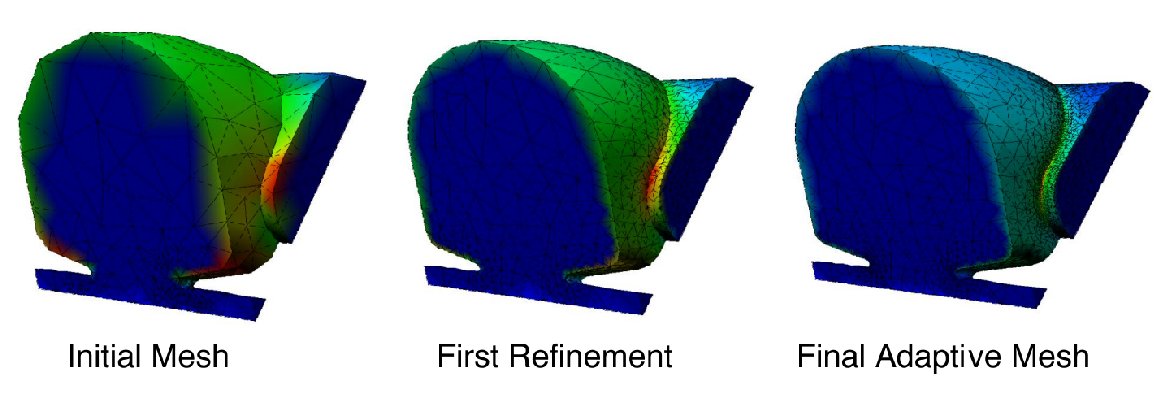
\epsfig{file=adapt-cavity.ps,width=10cm}
\caption{Adaptive analysis of a Trispal 4-petal accelerator cavity.}
\label{fig:trispalAdapt}
\end{center}
\end{figure}

\subsubsection{Metal Forming Simulation}

In 3D metal forming simulations, the workpiece undergoes large plastic
deformations that result in major changes in the domain geometry. The
meshes of the deforming parts typically need to be frequently modified
to continue the analysis due to large element distortions, mesh
discretization errors and/or geometric approximation errors. In these
cases, it is necessary to replace the deformed mesh with an improved
mesh that is consistent with the current geometry.  Procedures to
determine a new mesh size field considering each of these factors have
been developed and used in conjunction with local mesh modification
\cite{WaKo04}. The procedure includes functions to transfer history
dependent field variables as each mesh modification is performed
\cite{WaKo04}.

Figure~\ref{fig:forming} shows the set-up, initial mesh and final
adapted meshes for a steering link manufacturing problem solved using
the DEFORM-3D analysis engine \cite{Fl04} within a mesh
modification-based adaptive loop. A total stroke of 41.7mm is taken in
the simulation. The initial workpiece mesh consists 28,885
elements. The simulation is completed with 20 mesh modification steps
producing a final mesh with 102,249 elements.


\begin{figure}
\begin{center}
\epsfig{file=forming.ps,width=10cm}
\caption{Metal forming example.}
\label{fig:forming}
\end{center}
\end{figure}



\subsection{Mesh Quality Improvement}\label{sec:quality-improvement}

Mesh quality improvement techniques can be applied based on \em{a
priori} geometric quality metrics or \em{a posteriori} solution-based
metrics improvements.  Low-level mesh improvement operations include
vertex relocation, topology modification, vertex insertion, and vertex
deletion.  The relationship of the latter two with the TSTT interface is
discussed in Section~\ref{sec:adaptive-loop} of this paper.

The TSTT center is supporting the development of a stand-alone mesh
quality improvement toolkit, called Mesquite.  Mesquite currently
provides state-of-the-art algorithms for vertex relocation, and the
addition of topology modification is planned for the near future.
Mesquite is designed to be flexible enough to work on a wide array of
mesh types ranging from structured meshes to unstructured and hybrid
meshes and a number of different two and three dimensional element
types.

% Question for Lori:  Why does Mesquite need to know the number of
% elements of a given type or topology?

Vertex relocation schemes must operate on the surface of the geometric
domain as well as in the interior of the domain to fully optimize the
mesh.  As such, the software must have functional access to both the
high level description of the geometric domain and to individual mesh
entities such as element vertices.  In particular, to operate on
interior vertices, Mesquite queries a TSTT implementation for vertex
coordinate information, adjacency information, and the number of
elements of a given type or topology.  After determining the optimal
location for a vertex, Mesquite requests that the TSTT implementation
update vertex coordinate information.

To operate on the surface mesh, Mesquite must also use TSTT geometric
queries to determine the surface normal and the closest point on the
surface.  Explicit classification of the mesh vertex against a geometric
surface is required, as there are some cases for which the closest point
query will return a point on the wrong surface, resulting in inverted or
invalid meshes.

The TSTT center is also currently working to develop an interface for
simplicial mesh topology modification.  The topology modifications
planned for this interface are face and edge swapping operators.  A
reference implementation for this service based on the TSTT mesh
interface is also in progress, with the goal of enabling swapping in any
TSTT implementation supporting triangles (2D) or tetrahedra (3D).  

In gathering enough information to determine whether a swap is
desirable, any mesh topology modification scheme must make extensive use
of the TSTT entity adjacency and vertex coordinate retrieval functions.
Reconfiguring the mesh, when this is appropriate, requires deletion of
old entities and creation of new entities through the TSTT interface.
In addition, classification operators are again essential.  For
instance, reconfiguring tetrahedra that classify on different geometric
regions results in tetrahedra that do not classify on either region, so
this case must be avoided.  Likewise, classification checks make it easy
to identify and disallow mesh reconfigurations that would remove a mesh
edge classified on a geometric edge.

In addition to basic geometry, topology and classification information,
a TSTT implementation must provide additional information for mesh
improvement schemes to operate effectively and efficiently.  For
example, even for simple mesh improvement schemes, the implementation
must be able to indicate which entities may be modified and which may
not.  For mesh improvement schemes to operate on an entire mesh rather
than simply accepting requests entity by entity, a TSTT implementation
must support some form of iterator.  Furthermore, advanced schemes may
allow the user to input a desired size, orientation, degree of
anisotropy, or even an initial reference mesh; exploiting such features
will require the implementation to associate information of many
different types with mesh entities and pass that information to the mesh
improvement scheme when requested.


\begin{verbatim}
  - SLAC design optimization 
  - Front tracking
\end{verbatim}

\section{Conclusions/Future work}

\section{Current Status and Ongoing Work\label{sec:Conclusions}}

The TSTT mesh interface has been implemented into several existing
meshing tools, including FMDB (RPI), GRUMMP (UBC), MOAB (SNL), Frontier
(SUNY SB), Overture (LLNL), and NWGrid (PNNL).  The interface is used by
several TSTT-developed mesh services tools including a mesh quality
improvement toolkit (Mesquite)\cite{Mesquite03}, a face- and
edge-swapping service\cite{TSTT-swap-tool}, and a mesh adaptation service.  In
addition, the TSTT interface is used in several
application codes.  The most notable of these is the joint work between
the TSTT consortium and researchers at the Stanford Linear Accelerator
Center (SLAC).  In this work, researchers are developing the TSTT-based
mesh services needed in design optimization of accelerator cavities and
to insert a mesh adaptation loop into SLAC's linear accelerator design
code\cite{GeLe04}.

To increase the dissemination of TSTT-compliant tools, we are now
working to establish component-level compliance with the standards of
the Common Component Architecture (CCA) Forum\cite{cca-forum}.  The CCA
Forum is defining a component architecture tailored to address all
aspects of high-performance scientific computing.  As part of this
effort, they are creating the Rapid Application Development environment,
in which TSTT mesh implementations will play a key role.

Work continues to improve the functionality and ease of use of the TSTT
interface.  We are working to adapt our current unit test suite for full
TSTTM implementations for use by those requiring correct behavior for
only a subset of functionality to be able to use a particular service.
Also, we expect to leverage current Babel research aimed at improving
software component compliance and usage through interface-level software
contracts\cite{dahlgren:sehpcs04,dahlgren:study04,dahlgren:sehpcs05}.

More information on the TSTT interface, including complete documentation,
can be found at http://www.tstt-scidac.org.



\section*{Acknowledgments} 

\bibliographystyle{plain}
\bibliography{../biblio/tstt}

\end{document} 
